\chapter[\Coq{} Integrated Development Environment]{\Coq{} Integrated Development Environment\label{Addoc-coqide}
\ttindex{coqide}}
%HEVEA\cutname{coqide.html}

The \Coq{} Integrated Development Environment is a graphical tool, to
be used as a user-friendly replacement to \texttt{coqtop}. Its main
purpose is to allow the user to navigate forward and backward into a
\Coq{} vernacular file, executing corresponding commands or undoing
them respectively. % CREDITS ? Proof general, lablgtk, ...

\CoqIDE{} is run by typing the command \verb|coqide| on the command
line. Without argument, the main screen is displayed with an ``unnamed
buffer'', and with a file name as argument, another buffer displaying
the contents of that file. Additionally, \verb|coqide| accepts the same
options as \verb|coqtop|, given in Chapter~\ref{Addoc-coqc}, the ones having
obviously no meaning for \CoqIDE{} being ignored.

\begin{figure}[t]
\begin{center}
%HEVEA\imgsrc[alt="coqide main screen"]{coqide.png}
%BEGIN LATEX
\ifpdf   % si on est en pdflatex
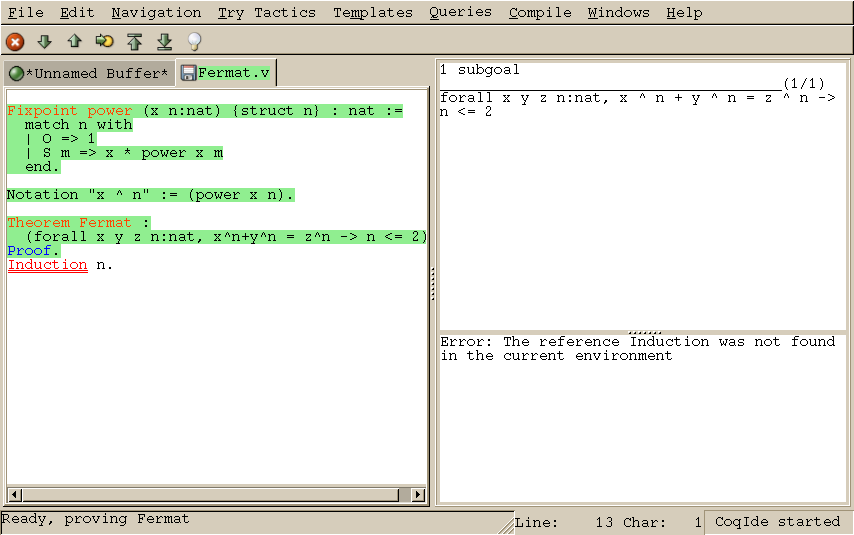
\includegraphics[width=1.0\textwidth]{coqide.png}
\else
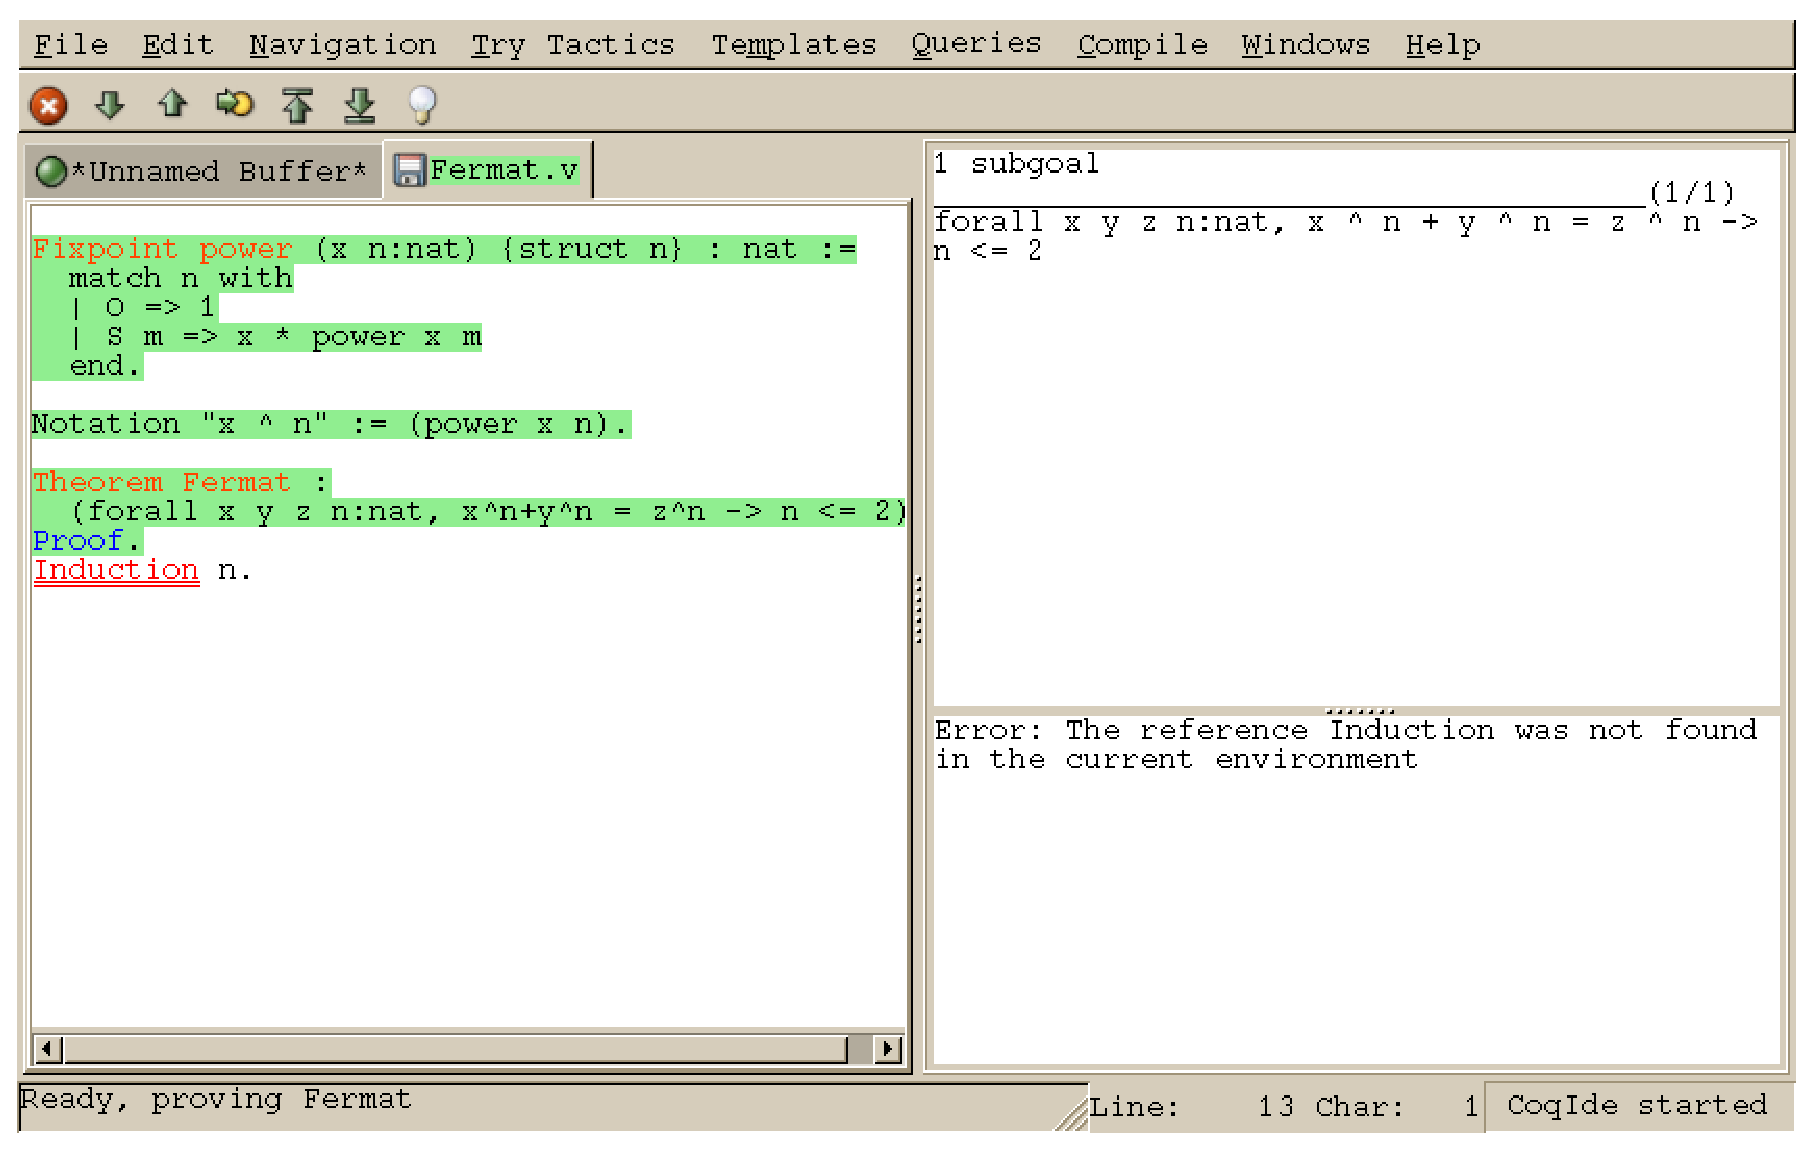
\includegraphics[width=1.0\textwidth]{coqide.eps}
\fi
%END LATEX
\end{center}
\caption{\CoqIDE{} main screen}
\label{fig:coqide}
\end{figure}

A sample \CoqIDE{} main screen, while navigating into a file
\verb|Fermat.v|, is shown on Figure~\ref{fig:coqide}.  At
the top is a menu bar, and a tool bar below it. The large window on
the left is displaying the various \emph{script buffers}. The upper right
window is the \emph{goal window}, where goals to
prove are displayed. The lower right window is the \emph{message window},
where various messages resulting from commands are displayed. At the
bottom is the status bar.

\section{Managing files and buffers, basic edition}

In the script window, you may open arbitrarily many buffers to
edit. The \emph{File} menu allows you to open files or create some,
save them, print or export them into various formats. Among all these
buffers, there is always one which is the current \emph{running
  buffer}, whose name is displayed on a green background, which is the
one where Coq commands are currently executed.

Buffers may be edited as in any text editor, and classical basic
editing commands (Copy/Paste, \ldots) are available in the \emph{Edit}
menu. \CoqIDE{} offers only basic editing commands, so if you need
more complex editing commands, you may launch your favorite text
editor on the current buffer, using the \emph{Edit/External Editor}
menu.

\section{Interactive navigation into \Coq{} scripts}

The running buffer is the one where navigation takes place. The
toolbar proposes five basic commands for this. The first one,
represented by a down arrow icon, is for going forward executing one
command. If that command is successful, the part of the script that
has been executed is displayed on a green background. If that command
fails, the error message is displayed in the message window, and the
location of the error is emphasized by a red underline.

On Figure~\ref{fig:coqide}, the running buffer is \verb|Fermat.v|, all
commands until the \verb|Theorem| have been already executed, and the
user tried to go forward executing \verb|Induction n|. That command
failed because no such tactic exist (tactics are now in
lowercase\ldots), and the wrong word is underlined.

Notice that the green part of the running buffer is not editable. If
you ever want to modify something you have to go backward using the up
arrow tool, or even better, put the cursor where you want to go back
and use the \textsf{goto} button. Unlike with \verb|coqtop|, you
should never use \verb|Undo| to go backward.

Two additional tool buttons exist, one to go directly to the end and
one to go back to the beginning. If you try to go to the end, or in
general to run several commands using the \textsf{goto} button, the
  execution will stop whenever an error is found.

If you ever try to execute a command which happens to run during a
long time, and would like to abort it before its
termination, you may use the interrupt button (the white cross on a red circle).

Finally, notice that these navigation buttons are also available in
the menu, where their keyboard shortcuts are given.

\section[Try tactics automatically]{Try tactics automatically\label{sec:trytactics}}

The menu \texttt{Try Tactics} provides some features for automatically
trying to solve the current goal using simple tactics. If such a
tactic succeeds in solving the goal, then its text is automatically
inserted into the script. There is finally a combination of these
tactics, called the \emph{proof wizard} which will try each of them in
turn. This wizard is also available as a tool button (the light
bulb).  The set of tactics tried by the wizard is customizable in
the preferences.

These tactics are general ones, in particular they do not refer to
particular hypotheses. You may also try specific tactics related to
the goal or one of the hypotheses, by clicking with the right mouse
button on the goal or the considered hypothesis. This is the
``contextual menu on goals'' feature, that may be disabled in the
preferences if undesirable.

\section{Proof folding}

As your script grows bigger and bigger, it might be useful to hide the proofs
of your theorems and lemmas.

This feature is toggled via the \texttt{Hide} entry of the \texttt{Navigation}
menu. The proof shall be enclosed between \texttt{Proof.} and \texttt{Qed.},
both with their final dots. The proof that shall be hidden or revealed is the
first one whose beginning statement (such as \texttt{Theorem}) precedes the
insertion cursor.

\section{Vernacular commands, templates}

The \texttt{Templates} menu allows using shortcuts to insert
vernacular commands. This is a nice way to proceed if you are not sure
of the spelling of the command you want.

Moreover, this menu offers some \emph{templates} which will automatic
insert a complex command like Fixpoint with a convenient shape for its
arguments.

\section{Queries}

\begin{figure}[t]
\begin{center}
%HEVEA\imgsrc[alt="coqide query window"]{coqide-queries.png}
%BEGIN LATEX
\ifpdf  % si on est en pdflatex
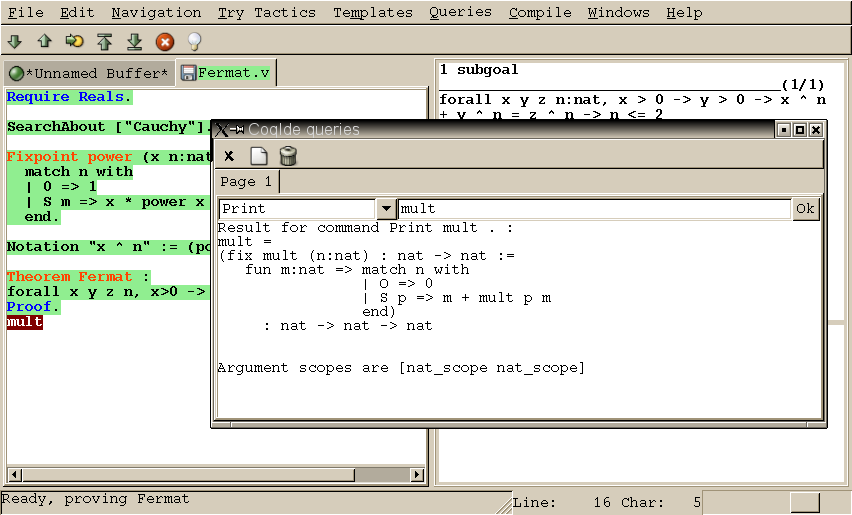
\includegraphics[width=1.0\textwidth]{coqide-queries.png}
\else
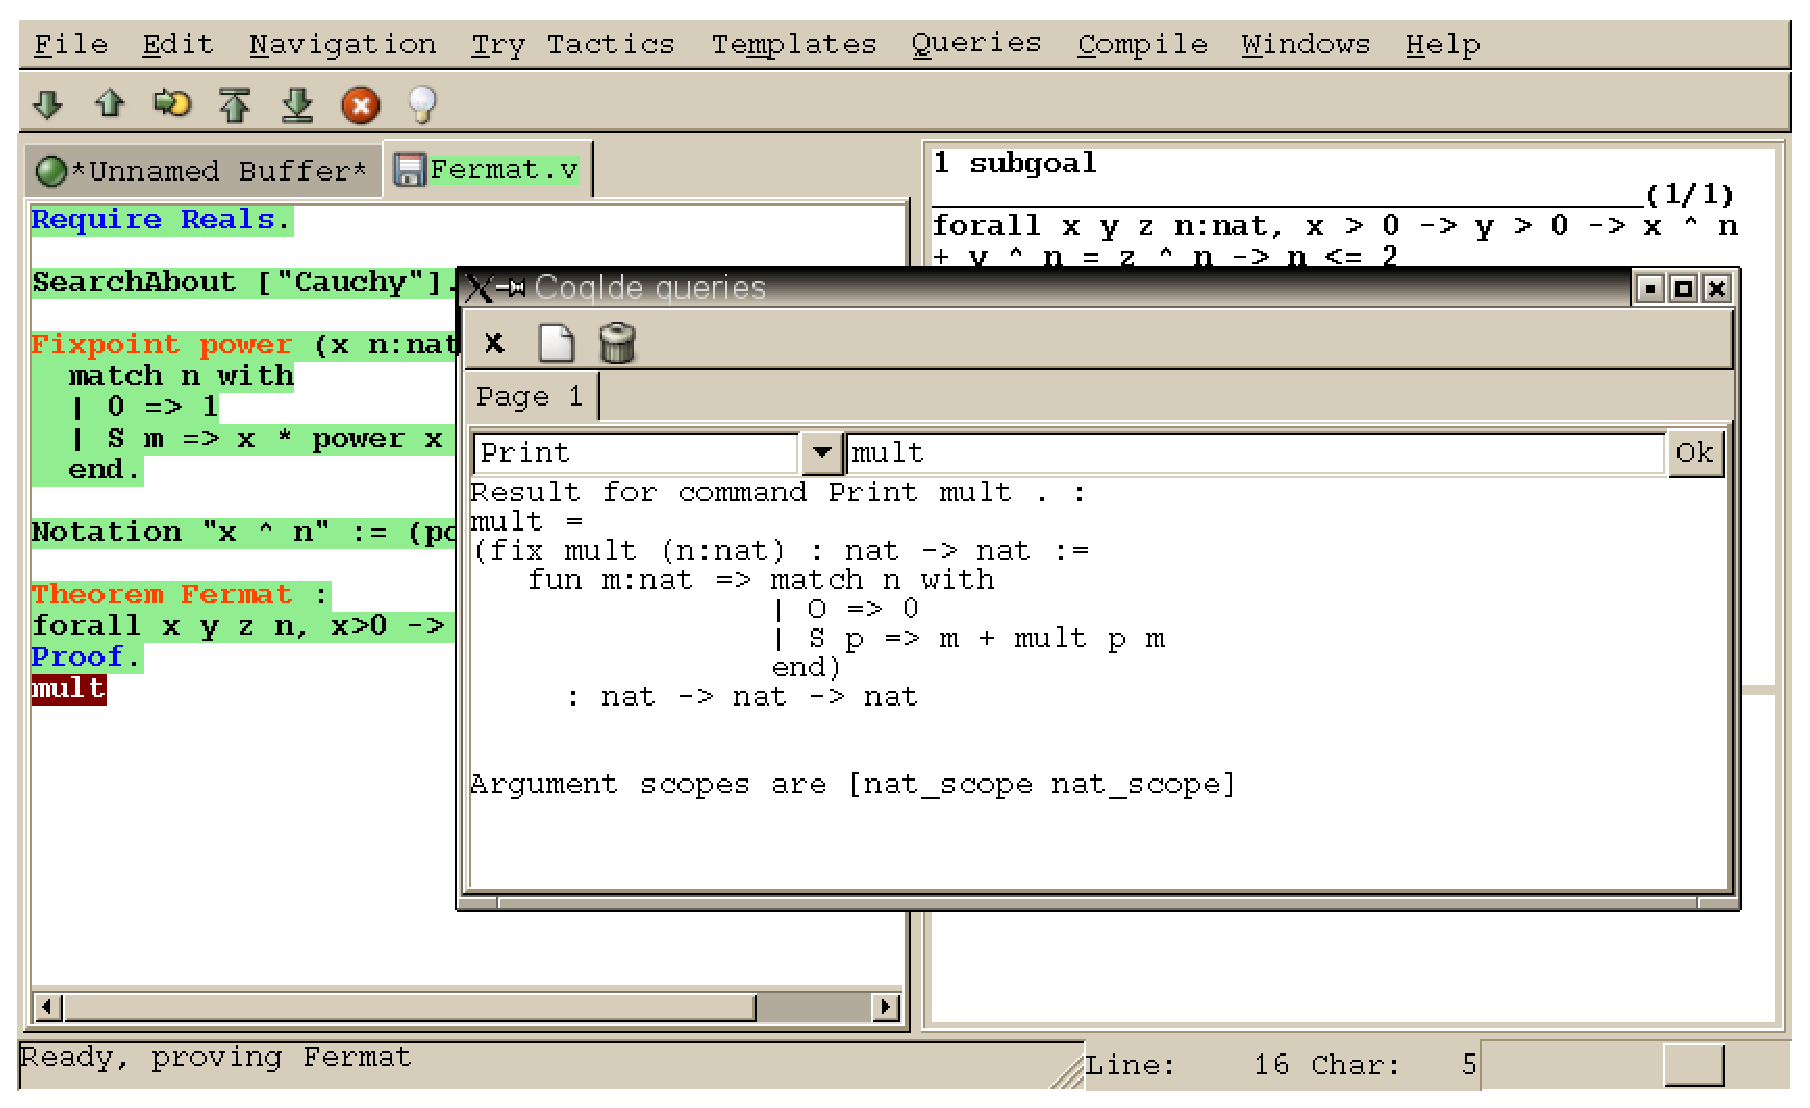
\includegraphics[width=1.0\textwidth]{coqide-queries.eps}
\fi
%END LATEX
\end{center}
\caption{\CoqIDE{}: the query window}
\label{fig:querywindow}
\end{figure}


We call \emph{query} any vernacular command that do not change the
current state, such as \verb|Check|, \verb|Search|, etc. Those
commands are of course useless during compilation of a file, hence
should not be included in scripts. To run such commands without
writing them in the script, \CoqIDE{} offers another input window
called the \emph{query window}. This window can be displayed on
demand, either by using the \texttt{Window} menu, or directly using
shortcuts given in the \texttt{Queries} menu. Indeed, with \CoqIDE{}
the simplest way to perform a \texttt{Search} on some identifier
is to select it using the mouse, and pressing \verb|F2|. This will
both make appear the query window and run the \texttt{Search} in
it, displaying the result. Shortcuts \verb|F3| and \verb|F4| are for
\verb|Check| and \verb|Print| respectively.
Figure~\ref{fig:querywindow} displays the query window after selection
of the word ``mult'' in the script windows, and pressing \verb|F4| to
print its definition.

\section{Compilation}

The \verb|Compile| menu offers direct commands to:
\begin{itemize}
\item compile the current buffer
\item run a compilation using \verb|make|
\item go to the last compilation error
\item create a \verb|makefile| using \verb|coq_makefile|.
\end{itemize}

\section{Customizations}

You may customize your environment using menu
\texttt{Edit/Preferences}. A new window will be displayed, with
several customization sections presented as a notebook.

The first section is for selecting the text font used for scripts, goal
and message windows.

The second section is devoted to file management: you may
configure automatic saving of files, by periodically saving the
contents into files named \verb|#f#| for each opened file
\verb|f|. You may also activate the \emph{revert} feature: in case a
opened file is modified on the disk by a third party, \CoqIDE{} may read
it again for you. Note that in the case you edited that same file, you
will be prompt to choose to either discard your changes or not. The
\texttt{File charset encoding} choice is described below in
Section~\ref{sec:coqidecharencoding}


The \verb|Externals| section allows customizing the external commands
for compilation, printing, web browsing. In the browser command, you
may use \verb|%s| to denote the URL to open, for example: %
\verb|mozilla -remote "OpenURL(%s)"|.

The \verb|Tactics Wizard| section allows defining the set of tactics
that should be tried, in sequence, to solve the current goal.

The last section is for miscellaneous boolean settings, such as the
``contextual menu on goals'' feature presented in
Section~\ref{sec:trytactics}.

Notice that these settings are saved in the file \verb|.coqiderc| of
your home directory.

A gtk2 accelerator keymap is saved under the name \verb|.coqide.keys|.
It is not recommanded to edit this file manually: to modify a given menu
shortcut, go to the corresponding menu item without releasing the
mouse button, press the key you want for the new shortcut, and release
the mouse button afterwards. If your system does not allow it, you may still
edit this configuration file by hand, but this is more involved.

\section{Using Unicode symbols}

\CoqIDE{} is based on GTK+ and inherits from it support for Unicode in
its text windows. Consequently a large set of symbols is available for
notations.

\subsection{Displaying Unicode symbols}

You just need to define suitable notations as described in
Chapter~\ref{Addoc-syntax}. For example, to use the mathematical symbols
$\forall$ and $\exists$, you may define
\begin{quote}\tt
Notation "$\forall$ x : t, P" := \\
\qquad  (forall x:t, P) (at level 200, x ident).\\
Notation "$\exists$ x : t, P" := \\
\qquad  (exists x:t, P) (at level 200, x ident).
\end{quote}
There exists a small set of such notations already defined, in the
file \verb|utf8.v| of \Coq{} library, so you may enable them just by
\verb|Require utf8| inside \CoqIDE{}, or equivalently, by starting
\CoqIDE{} with \verb|coqide -l utf8|.

However, there are some issues when using such Unicode symbols: you of
course need to use a character font which supports them. In the Fonts
section of the preferences, the Preview line displays some Unicode symbols, so
you could figure out if the selected font is OK. Related to this, one
thing you may need to do is choose whether GTK+ should use antialiased
fonts or not, by setting the environment variable \verb|GDK_USE_XFT|
to 1 or 0 respectively.

\subsection{Defining an input method for non ASCII symbols}

To input a Unicode symbol, a general method provided by GTK+
is to simultaneously press the
Control, Shift and ``u'' keys, release, then type the hexadecimal code of the
symbol required, for example \verb|2200| for the $\forall$ symbol.
A list of symbol codes is available at \url{http://www.unicode.org}.

An alternative method which does not require to know the hexadecimal
code of the character is to use an Input Method Editor. On POSIX
systems (Linux distributions, BSD variants and MacOS X), you can use
\texttt{uim} version 1.6 or later which provides a \LaTeX{}-style
input method.

To configure \texttt{uim}, execute \texttt{uim-pref-gtk} as your regular user.
In the "Global Settings" group set the default Input Method to "ELatin" (don't
forget to tick the checkbox "Specify default IM"). In the "ELatin" group set the
layout to "TeX", and remember the content of the "[ELatin] on" field (by default
Control-\textbackslash). You can now execute CoqIDE with the following commands (assuming
you use a Bourne-style shell):

\begin{verbatim}
$ export GTK_IM_MODULE=uim
$ coqide
\end{verbatim}

Activate the ELatin Input Method with Control-\textbackslash, then type the
sequence "\verb=\Gamma=". You will see the sequence being
replaced by $\Gamma$ as soon as you type the second "a".

\subsection[Character encoding for saved files]{Character encoding for saved files\label{sec:coqidecharencoding}}

In the \texttt{Files} section of the preferences, the encoding option
is related to the way files are saved.

If you have no need to exchange files with non UTF-8 aware
applications, it is better to choose the UTF-8 encoding, since it
guarantees that your files will be read again without problems. (This
is because when \CoqIDE{} reads a file, it tries to automatically
detect its character encoding.)

If you choose something else than UTF-8, then missing characters will
be written encoded by \verb|\x{....}| or \verb|\x{........}| where
each dot is an hexadecimal digit: the number between braces is the
hexadecimal Unicode index for the missing character.


%%% Local Variables:
%%% mode: latex
%%% TeX-master: "Reference-Manual"
%%% End:
